%
% box.tex
%
% (c) 2018 Prof Dr Andreas Müller, Hochschule Rapperswil
%
\section{Ein Modell für die thermohaline Zirkulation}
\rhead{Ein Modell für die thermohaline Zirkulation}
Jedes numerische Modelle der Zirkulation basiert auf einer Diskretisation
des Gebietes.
Der Ozean wird also in kleine Teilgebiete aufgeteilt.
Gesucht sind Temperatur und Salinität in jedem Teilgebiet.
Dann werden Gleichungen aufgestellt, die den Austausch von Salz und
Wärme zwischen den Teilgebieten beschreiben.
Die Lösung dieser Gleichungen wird uns das Ausmass der Zirkulation zeigen
und erlauben abzuschätzen, wie sich die Zirkulation ändert, wenn sich
die äusseren Bedinungen verschieben.

\subsection{Ein einfaches Box-Modell}
Um einen ersten Eindruck von der Dynamik der thermohalinen Zirkulation
zu erhalten, verwenden wir ein Modell mit genau zwei Teilgebieten.
Wir modellieren den Atlantik nördlich des Äquators als zwei Gebiete.
Gebiet 1 ist das Polargebiet mit typischerweise tieferen Temperaturen,
Gebiet 2 ist das Gebiet in der Nähe des Äquators.
In jedem dieser Gebiet modellieren wir nur das Wasser, welches tatsächlich
von der Zirkulation umgewälzt wird.
Wir nehmen an, dass es sich durch die zwei Parameter Temperatur und
Salinität beschreiben lässt.
Wir nennen die Variablen im Gebiet $i$ $T_i$ und $S_i$.

Das Wasser welches an der Zirkulation teilnimmt ist umgeben von einem
viel grösseren Wasserreservoir, welches mit dem strömenden Wasser 
im Wärme- und Salzaustausch steht.
Wir bezeichnen die konstanten Parameter dieses Reservoirs mit
$T_i^*$ und $S_i^*$.
In Abbildung~\ref{skript:boxmodell-blid} sind die beiden Gebiete
grau dargestellt, das in Zirkulation befindliche Wasser hellblau.
\begin{figure}
\centering
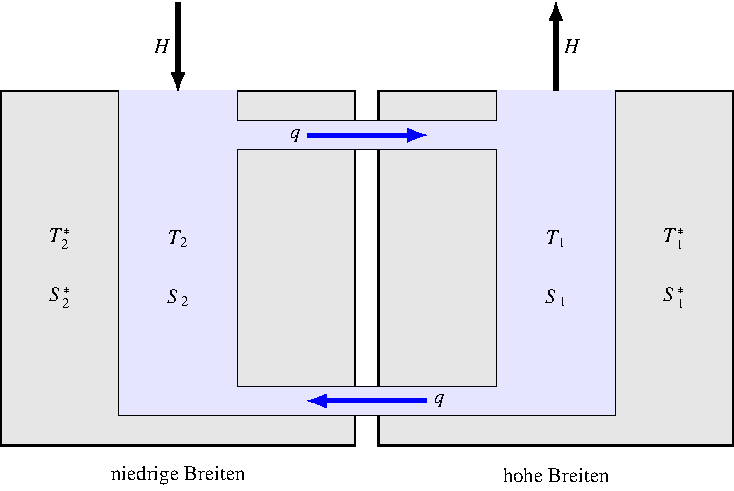
\includegraphics{chapters/4/boxmodell.pdf}
\caption{Einfaches Modell der thermohalinen Zirkulation
\label{skript:boxmodell-bild}}
\end{figure}

Die Zirkulation ist charakterisiert durch den Massefluss $q$ der
Tiefenströmung.
Da kein Wasser verloren gehen kann, muss in Oberflächennähe der gleiche
Fluss herrschen.
Da auch kein Salz verloren gehen kann, müssen sich auch die Salzflüsse
zwischen den beiden Gebieten ausgleichen.
Die Salinität wird zum Beispiel durch die Verdunstung erhöht, während
Niederschlag sie erniedrigt.
Süsswasserflüsse von Kontinenten reduzieren ebenfalls die Salinität.
Dies bedeutet, dass zusätzlich zum Massestrom $q$ ein virtueller 
Salzstrom zwischen den beiden Gebieten herrscht, den wir mit $H$ bezeichnen.

\subsection{Modell-Gleichungen}
Wir müssen jetzt Differentialgleichungen aufstellen, welche die
zeitliche Entwicklung von Temperatur $T_i(t)$ und Salinität $S_i(t)$
beschreiben kann.
Die Temperaturentwicklung wird bestimmt einerseits durch den Energietransport
durch den Fluss $q$ und andererseits durch den Wärmeaustausch mit dem
umgebenden Wasser.
Der Fluss $q$ hat zur Folge, dass sich die Temperaturen $T_1$ und $T_2$
angleichen.
Die beiden Flüsse oben und unten in Abbildung~\ref{skript:boxmodell-bild}
transportieren die gleiche Menge Wasser pro Zeiteinheit.
Es wird also gleichviel Wasser mit Temperatur $T_1$ ins Gebiet $2$ 
transportiert wie Wasser mit Temperatur $T_2$ ins Gebiet $1$.
Das Vorzeichen von $q$ spielt dabei keine Rolle, denn ändert das
Vorzeichen von $q$, fliesst das Wasser mit Temperatur $T_1$ einfach
durch den anderen Kanal.
Die Temperaturänderung von $T_1$ ist also propoertional zu $|q|(T_2-T_1)$.

Der Wärmeaustausch mit dem umgebenden Wasser ist proportional zur
Temperaturdifferenz, wir bezeichnen den Proportionalitätsfaktor mit $c$.
\begin{equation}
\begin{aligned}
\frac{dT_1}{dt}
&=
c(T_1^*-T_1)
+
|q|(T_2-T_1)
\\
\frac{dT_2}{dt}
&=
c(T_2^*-T_2)
+
|q|(T_1-T_2).
\end{aligned}
\label{skript:thc:temperaturgleichung}
\end{equation}

Analoge Überlegungen müssen wir jetzt auch noch für die Salinität anstellen.
Der Ausgleich der Salinität $S_i$ mit der Salinität $S_i^*$ des
umgebenden Meersbeckens ist propertional zur Differenz, der
Proportionalitätsfaktor, den wir mit $d$ bezeichen, ist bestimmt durch
die Diffusionsgeschwindigkeit und die turbulente Durchmischung des
zirkulierenden Wassers mit der Umgebung.
Dazu kommt noch der virtuelle Salzfluss $H$:
\begin{equation}
\begin{aligned}
\frac{dS_1}{dt}
&=
\phantom{-}
H
+
d(S_1^*-S_1)
+
|q|(S_2-S_1)
\\
\frac{dS_2}{dt}
&=
-H
+
d(S_2^*-S_2)
+
|q|(S_1-S_2).
\end{aligned}
\label{skript:thc:salinitaetsgleichung}
\end{equation}
Man beachte, dass die Temperaturgleichungen~\ref{skript:thc:temperaturgleichung}
und die Salinitätsgleichungen~\ref{skript:thc:salinitaetsgleichung} 
gekoppelt sind, da der Fluss $q$ angetrieben wird vom Dichteunterschied,
der wiederum von Temperatur und Salinität abhängt.

\subsection{Antrieb der Zirkulation}
Die Zirkulation wird wie gesagt vom Dichteunterschied angetrieben.
Es gibt also einen Proportionalitätsfaktor $k$ derart, dass
\[
q = k\frac{\varrho_1 - \varrho_2}{\varrho_0}.
\]
Setzt man die Formel~\ref{skript:salinity-linear} ein, findet man
\[
q
=
k(-\alpha(T_1-T_2) + \beta(S_1-S_2))
=
k(\alpha(T_2-T_1) + \beta(S_1-S_2))
=
k(\alpha(T_2-T_1) - \beta(S_2-S_1)).
\]
Schreiben wir $\Delta T = T_2-T_1$ und $\Delta S=S_2-S_1$,
dann ist der Fluss nur von den Differenzen abhängig
\begin{equation}
q=k(\alpha\Delta T-\beta\Delta S).
\label{skript:thc:fluss-delta}
\end{equation}

\subsection{Anomalie-Gleichungen}
Die absoluten Werte von $T_i$ und $S_i$ sind nicht wirklich wichtig,
viel wichtiger sind die Unterschiede $\Delta T_i$ und $\Delta S_i$.
Verschwinden die Differenzen, kommt die Zirkulation zum erliegen,
und dies sind die Phänomene, die wir mit den Gleichungen prognostizieren
können möchten.
Wir streben daher an, die Gleichungen
\eqref{skript:thc:temperaturgleichung}
und
\eqref{skript:thc:salinitaetsgleichung}
in eine Form zu bringen, die nur von Differenzen und Anomalien
abhängt.

Wir schreiben
\[
T_0
=
\frac12(T_1+T_2)
\qquad\text{und}\qquad
S_0
=
\frac12(S_1+S_2)
\]
für die Mittelwerte von Temperatur und Salinität.
Indem wir den Mittelwert der Temperaturgleichungen
\eqref{skript:thc:temperaturgleichung}
bzw.~der Salinitätsgleichung \eqref{skript:thc:salinitaetsgleichung} bilden,
bekommen wir die Gleichungen
\begin{equation}
\begin{aligned}
\frac{dT_0}{dt}
&=
c(T_0^*-T_0)
\\
\frac{dS_0}{dt}
&=
d(S_0^*-S_0),
\end{aligned}
\label{skript:thc:mittelgleichung}
\end{equation}
wobei $T_0^* = \frac12(T_1^*+T_2^*)$ und $S_0^* = \frac12(S_1^*+S_2^*)$.
Die Differentialgleichungen~\ref{skript:thc:mittelgleichungen} 
besagen, dass die mittlere Temperatur des zirkulierenden Wassers
gegen die mittlere Temperatur des umliegenden Meeresbeckens strebt.

Da die Mitteltemperatur langfristig gegen die Mitteltemperatur der
umliegenden Meeresbecken strebt liegt es nahe, Temperatur und
Salinität auf diese Mitteltemperatur zu beziehen.
Wir ersetzen also
\begin{equation}
\begin{aligned}
\bar T_1&=T_1-T_0^*,
&
\bar T_2&=T_2-T_0^*
&&\Rightarrow&
\bar T_0&=T_0-T_0^*
\\
\bar S_1&=S_1-S_0^*,
&
\bar S_2&=S_2-S_0^*
&&\Rightarrow&
\bar S_0&=S_0-S_0^*
\end{aligned}
\end{equation}
Die Differentialgleichungen~\eqref{skript:thc:mittelgleichung}
für die Mittelwerte wird damit zu
\begin{align*}
\frac{d\bar T_0}{dt} &= -c \bar T_0\\
\frac{d\bar S_0}{dt} &= -d \bar S_0.
\end{align*}
Die Differentialgleichungen für
$T_i=\bar T_i + T_0^*$
und
$S_i=\bar S_i + S_0^*$
sind
\begin{align*}
\frac{dT_i}{dt}
&=
\frac{d\bar T_i}{dt}
=
c(T_i^*-T_i)
+ |q|\Delta \bar T
=
c(T_i^*- \bar T_i - T_0^*)
+ |q|\Delta \bar T
\\
\frac{dS_i}{dt}
&=
\frac{d\bar S_i}{dt}
=
\pm H
+
d(S_i^*-S_i)
+ |q|\Delta \bar S
=
\pm H
+
d(S_i^*- \bar S_i - S_0^*)
+ |q|\Delta \bar S
\end{align*}
Die Differenzen $T_i^*-T_0^*$ und $S_i^*-S_0^*$ können wir vereinfacht
als
\begin{align*}
T_1^*-T_0^* 
&=
T_1^* - \frac12(T_2^*-T_1^*)
=
-\frac12(T_2^*-T_1^*)
=
-T^*
\\
T_2^*-T_0^*
&=
T_2^*-\frac12(T_2^*-T_1^*)
=
\frac12(T_2^*-T_1^*)
=
T^*
\end{align*}
schreiben und analog für $S^*=\frac12(S_2^*-S_1^*)$.
Damit werden die Differentialgleichungen zu
\begin{equation}
\begin{aligned}
\frac{d\bar T_1}{dt}
&=
c(-T^*-\bar T_1) + |q| (\bar T_2-\bar T_1)
\\
\frac{d\bar T_2}{dt}
&=
c(T^*-\bar T_2) + |q| (\bar T_1-\bar T_2)
\\
\frac{d\bar S_1}{dt}
&=
-H
+
d(-S^*-\bar S_1) + |q|(\bar S_2 - \bar S_1)
\\
\frac{d\bar S_2}{dt}
&=
\phantom{-}H
+
d(S^*-\bar S_2) + |q|(\bar S_1 - \bar S_2)
\end{aligned}
\label{skript:thc:anomaliegleichungen}
\end{equation}
Man beachte, dass die $T^*$ und $S^*$ konstant sind.

In den Gleichungen~\eqref{skript:thc:anomaliegleichungen} hängt
$q$ von den Temperatur- und Salinitätsdifferenzen ab.
Wegen $\Delta\bar T=\Delta T$ und $\Delta\bar S$ ist nach
\eqref{skript:thc:fluss-delta}
\begin{equation}
q = k(\alpha\Delta\bar T-\beta \Delta\bar S).
\label{skript:thc:fluss-delta-anomalie}
\end{equation}

\subsection{Differenzgleichungen}
Wir können die Anomaliegleichungen \eqref{skript:thc:anomaliegleichungen}
noch etwas weiter umformen und die einzelnen Anomalien vollständig durch
die Differenzen ersetzen.
Die Differenzen und Summen der Gleichungen sind
\begin{equation}
\begin{aligned}
\frac{d\Delta\bar T}{dt}
&=
c(2T^*-\Delta\bar T)-2|q|\Delta\bar T
&&\qquad&
\frac{d\bar T_0}{dt}
&=
-c\bar T_0
\\
\frac{d\Delta\bar S}{dt}
&=
2H+d(2S^*-\Delta\bar S) - 2|q|\Delta\bar S
&&\qquad&
\frac{d\bar S_0}{dt}
&=
-d\bar S_0.
\end{aligned}
\label{skript:thc:differenzgleichungen}
\end{equation}
Die Gleichungen rechts drücken aus, dass die mittleren Anomalien
exponentiell gegen $0$ gehen.
Die linken Gleichungen beschreiben die Zeitentwicklung der Differenz
der Anomalien.
Man beachte, dass $q$ ebenfalls von den Anomalie-Differenzen abhängt.

\subsection{Zeitkonstanten}
\label{skript:thc:zeitkonstanten}
Der Koeffizienten $c$ beschreibt, wie schnell der Temperaturausgleich
durch Wärmeleitung oder turbulente Durchmischung erfolgt.
Der Koeffizient $d$ beschreibt, wie schnell der Salinitätsausgleich
durch Durchmischung und Diffusion stattfinden kann.
Je grösser diese Koeffizienten, desto schneller erfolgt der Prozess.
In den rechten Gleichungen von \eqref{skript:thc:differenzgleichungen}
ist dies ganz offensichtlich.
Vernachlässigen wir für den Moment den Einfluss der Zirkulation,
was wir durch $k=0$ im Ausdruck für $q$ beschreiben können, dann
sehen wir, dass die Differenzgleichungen beide von der Form
einer linearen inhomogenen Differentialgleichung
\[
\frac{d\Delta X}{dt}
=
X^* -cX
\]
sind, wobei $X^*$ eine Konstante ist.
Die Lösung der Gleichung ist
\[
X(t) = \frac{X^*}{c} + C_0 e^{-ct}
\]
mit einer Konstanten $C_0$, die aus den Anfangsbedingungen zu
bestimmen ist.
Die Terme $T^*$, $S^*$ und $H$ verschieben also nur die Lösung,
die Differenzen $\Delta\bar T$ und $\Delta\bar S$ streben exponentiell
wie $e^{-ct}$ bzw.~$e^{-dt}$ gegen diese Gleichgewichtswerte.

Die Grössen $1/c$ und $1/d$ haben die Dimension einer Zeit, wir nennen
sie die {\em Zeitkonstanten} des Prozesses, den $c$ bzw.~$d$ beschreiben.
\index{Zeitkonstante}
Ist zum Beispiel die Zeitkonstante $1/c$ der Temperatur sehr viel kleiner
als die Zeitkonstanten $1/d$ der Salinität, dann bedeutet dies, dass
sich die Temperaturdifferenzen sehr viel schneller ausgleichen als die
Salinitätsdifferenzen.
Für die langfristige Entwicklung der Zirkulation ist in diesem Fall
die Salinitätsentwicklung ausschlaggebend, die Temperaturfunktionen
können durch kosntante ersetzt werden.




